\section{Signal Extraction}
\label{Signal Extraction}
The total number of $\jpsi$ and $\psitwos$ signals is determined from an extended unbinned maximum 
likelihood fit to the invariant mass distribution of the selected candidates. The fit models for both $\jpsi$ 
and $\psitwos$ are the same, which we consider the previous studies of $\jpsi$ production at 13 TeV~\cite{LHCb-PAPER-2015-037} 
and $\psitwos$ production at 13 TeV~\cite{LHCb:2019eaj}. The only strategy for both is as follows.

In the fit the component of the background is modelled with an exponential function
\begin{equation}
f_{\rm bkg}(m)=a_0e^{-p_0\cdot m}.
\end{equation}
The signal component is described by the sum of two Crystal Ball (CB) functions~\cite{Skwarnicki:1986xj}.
The CB function is defined as:
\begin{equation}
 f_{\mathrm{CB}}(m;\mu,\sigma,\alpha,n) = 
 \begin{cases} 
      %\frac{\Big(\frac{n}{|\alpha|}\Big)^n e^{-\frac{1}{2}\alpha^2}}{(\frac{n}{|\alpha|}-|\alpha|-\frac{m-\mu}{\sigma})^n} & \frac{m-\mu}{\sigma} < -|\alpha|\\
      \Big(\frac{n}{|\alpha|}\Big)^n e^{-\frac{1}{2}\alpha^2} (\frac{n}{|\alpha|}-|\alpha|-\frac{m-\mu}{\sigma})^{-n} & \frac{m-\mu}{\sigma} < -|\alpha|\\
   \exp\Bigg( -\frac{1}{2}\Big(\frac{m-\mu}{\sigma}\Big)^2\Bigg) & \frac{m-\mu}{\sigma}>-|\alpha|.
\end{cases},
\end{equation}
which combines a Gaussian core (described by the parameters $\mu$ and $\sigma$) and one tail on the left (described by the parameters $\alpha$ and $n$).
The tails in CB functions are used to model the radiative effects, which leads to more candidates with lower invariant masses.
Not all parameters of the CB functions are free when fitting data. 
Some parameters are fixed or parameterized.
For both $\jpsi$ and $\psitwos$, the two CB functions share one common mean value $\mu$ and have different widths $\sigma_1$ and $\sigma_2$, and $\alpha$ is parametrized from simulation as a function of the $\sigma$:
$\alpha=2.066\pm0.0085\sigma-0.00011\sigma^2$, which applies to both CB functions. Furthermore, for $\psitwos$ only, $\sigma_1$ and $\sigma_2$ are parameterized as a linear function: $\sigma_2=25.7+\sigma_1$ and the fraction of the narrower CB function is fixed at 0.96. 
For the tail parameters, $n$ is fixed to unity from physics~\cite{LefrancoisTalk}.
%is used for different kinematic bins of \psitwos.
Therefore, there are merely two free parameters for the signal shape, $\mu$ and $\sigma_1$. The strategy followed the previous study of $\jpsi$ and $\psitwos$ production at 13 TeV~\cite{LHCb-PAPER-2015-037,LHCb:2019eaj}.
The invariant mass fit is performed in each $\pt-y$ and PVNTRACKS bin of the candidate.

\subsection{Determination of the prompt and detached signal yields}
\label{sec:MassTzFit}
To determine the signal yields of prompt and from-\bquark components separately, the $t_z$ distribution is used.
In each kinematic and multiplicity bin, an unbinned extended maximum likelihood fit to the two-dimension distributions of invariant mass $m(\mumu)$ and $t_z$ is performed to separate prompt component from that from \bquark.

At the generator level, the $t_z$ distribution of the prompt component is a Dirac delta function, $\delta(t_z)$, while that from $\bquark$ follows an exponential function as seen from simulation. 
For \jpsi and \psitwos signals, the detector resolution is taken into account by convolving a resolution function, which is described by the sum of two Gaussian functions,
\begin{equation}
f_\mathrm{resolution}(t_z;\mu,S_1,S_2,\beta) = \frac{\beta}{\sqrt{2\pi}S_1\sigma} e^{-\frac{(t_z-\mu)^2}{2S_1^2\sigma^2}}
+\frac{1-\beta}{\sqrt{2\pi}S_2\sigma} e^{-\frac{(t_z-\mu)^2}{2S_2^2\sigma^2}}.
\end{equation}
The parameter $\sigma$ is the event-by-event uncertainty of $t_z$, calculated by combining the estimated uncertainties of the \jpsi and \psitwos decay vertex and the associated PV.
Besides,$S_1$ and $S_2$ are two scale factors to correct the non-perfect estimation of the $t_z$ uncertainty, the parameter $\mu$ is the bias of the $t_z$ measurement, and $\beta$ is the fraction of one of the two Gaussians. 
In the fitting procedure, all the resolution parameters are floated.
For some (\pt,$y$, PVNTRACKS) bin, the count for signal yield for \psitwos or \jpsi is significantly low that fit will fail for too many free parameters, and we may set $\beta=0$, which is, only one Gaussian function is used to describe the resolution. 

It is possible that the reconstructed candidate is associated with a "wrong" PV. 
This can happen either because the real PV that produces the candidate failed to be reconstructed, and the candidate was associated with the nearest reconstructed PV in the event, or because a wrong PV is accidentally close to the candidate.
For the latter case, the positions of the reconstructed and the true PV are correlated, which results in a Gaussian-like $t_z$ distribution with a width much larger than the detection resolution. 
This effect can be described by adding a third Gaussian with a much larger width than the resolution function. 
However, it is found from simulation that including the wide Gaussian in the resolution does not change the fitted parameters significantly because the fraction of this component is quite small, $\leq 1\%$ as seen from studies in Ref.\cite{LHCb-PAPER-2015-037}.
Therefore, the third wide Gaussian is not used in the fit function.
For the former case that the true PV is not reconstructed, the true PV and wrongly associated PV are not correlated, which results in a long tail in the $t_z$ distribution that can be modeled using the next-event method for both \jpsi and \psitwos. 
The next-event method is applied directly on data sample. 
The next-event pseudo-proper time, $t_z^\mathrm{next}$, for each candidate, is calculated combining the candidate with the closest PV of another (next) event as
\begin{equation}
t_z^\mathrm{next}=\frac{(z_{\mu\mu}-z_\mathrm{PV}^\mathrm{next})\times m_{\mu\mu}}{p_z},
\end{equation}
where $z_\mathrm{PV}^\mathrm{next}$ is the $z$-coordinate of the nearest PV of the next selected event. 
The tail distribution is extracted in each bin separately and not convolved with resolution functions since the distribution is much wider than the resolution and very smooth in the whole $t_z$ region.
It should be noted that since the requirement of PV reconstruction is loose, using at least 4 VELO tracks, the probability to reconstruct the true PV is very high ($>99\%$). 

The candidates in the mass sidebands, where $m_{\mumu}$ is at least 60 $\mevc$ away from the mass of $\jpsi$ and $\psitwos$, are used as the background control sample to model the $t_z$ distribution of the background.
The background control sample consists of random combinations of muons from semi-leptonic $\bquark$ and $\cquark$ decays, which tend to produce positive $t_z$ values, as well as mis-reconstructed tracks from decays-in-flight of kaons and pions, which contribute both to positive and negative $t_z$ values.
The $t_z$ distribution of the background is therefore modeled with an empirical function, composed of a Dirac delta function and five exponentials (three for positive $t_z$ and two for negative $t_z$, with one positive $t_z$ and one negative sharing the same slope parameter). 
This function is convolved with the sum of two Gaussian functions as a resolution function, which has different parameters as for signals,\footnote{The uncertainty on the background vertex is usually worse than that for the signal vertex. } ,
\begin{align}
f_\mathrm{background} &=
\left[(1-f_1-f_2-f_3-f_4)\delta(t_z)+\theta(t_z)(\frac{f_1}{\tau_1}e^{-t_z/\tau_1}+\frac{f_2}{\tau_2}e^{-t_z/\tau_2})\right.
\nonumber\\
&\left. +\theta(-t_z)\frac{f_3}{\tau_3}e^{t_z/\tau_3}+\frac{f_4}{2\tau_4}e^{-|t_z|/\tau_4}
\right]\ast \left(\frac{\beta'}{\sqrt{2\pi}S^{'}_1\sigma} e^{-\frac{(t_z-\mu)^2}{2S^{'2}_1\sigma^2}}
  +\frac{1-\beta'}{\sqrt{2\pi}S^{'}_2\sigma} e^{-\frac{(t_z-\mu)^2}{2S^{'2}_2\sigma^2}}\right). 
\label{eq:TzBKG}
\end{align}
The parameters in Eq.~\ref{eq:TzBKG} are determined by fitting the $t_z$ distribution of background control sample defined above (in each kinematical bin of \jpsi and \psitwos), and are fixed for the final fits. 
In Fig.~\ref{fig:TzBKG}, the $t_z$ distribution of the background in the kinematic range $\pt\in[2,4]\gevc$, $y\in[2.0,2.8]$ and PVNTRACKS $\in[20,40]$ is shown, superposed by a fit using Eq.~\ref{eq:TzBKG}. 
%In Tables \ref{tab:tzbkgFitResults0}, \ref{tab:tzbkgFitResults1}, \ref{tab:tzbkgFitResults2}, \ref{tab:tzbkgFitResults3} and \ref{tab:tzbkgFitResults4}, all the background parameters in $t_z$ fits are given in each kinematic bin. 
%%%%%%%%%%%%%%%%%%%%%%%%%%%%%%%%%%%%%%%%%%%%%%%%%%%%%%%%%%%
\begin{figure}[!tbp]
   \begin{center}
     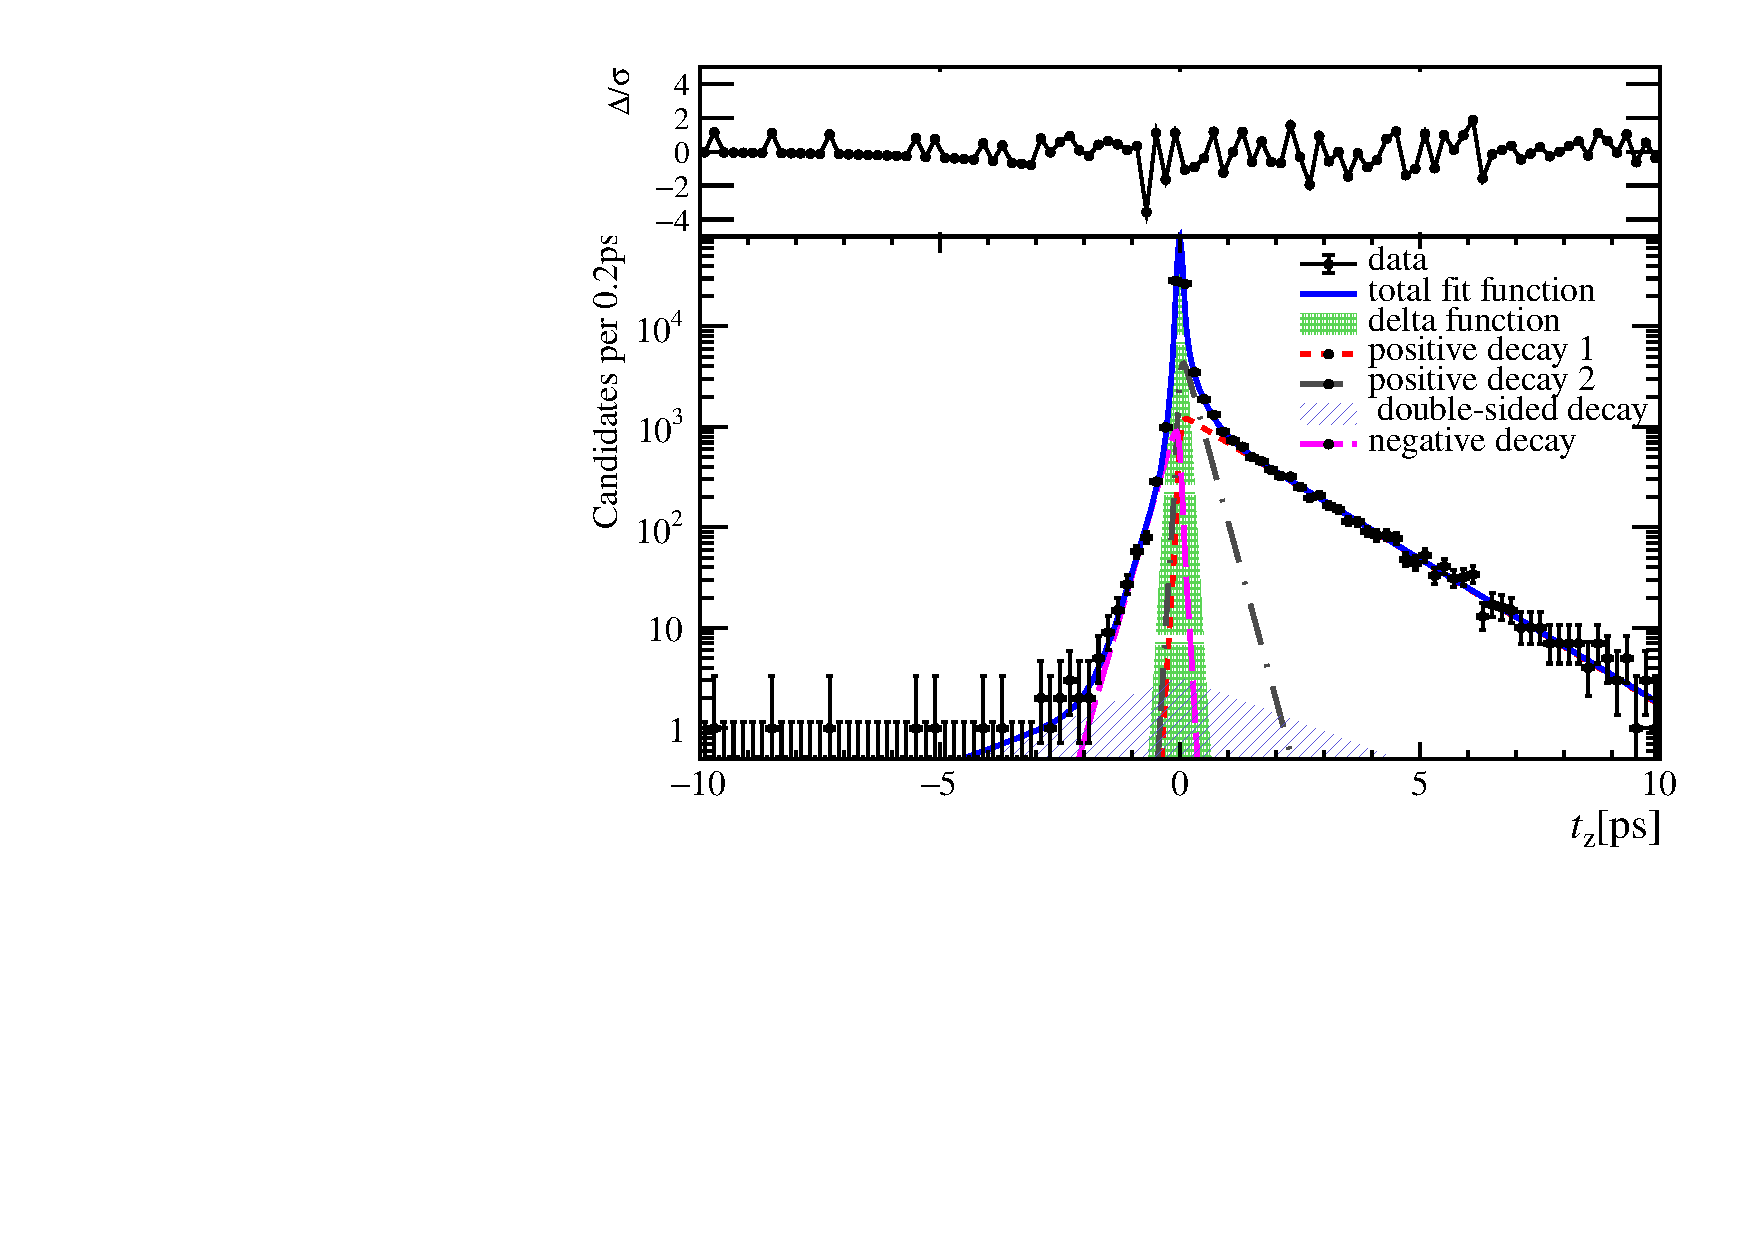
\includegraphics[width=0.49\linewidth]{pdf/Jpsi/Tzbkg/n2y1pt2}
     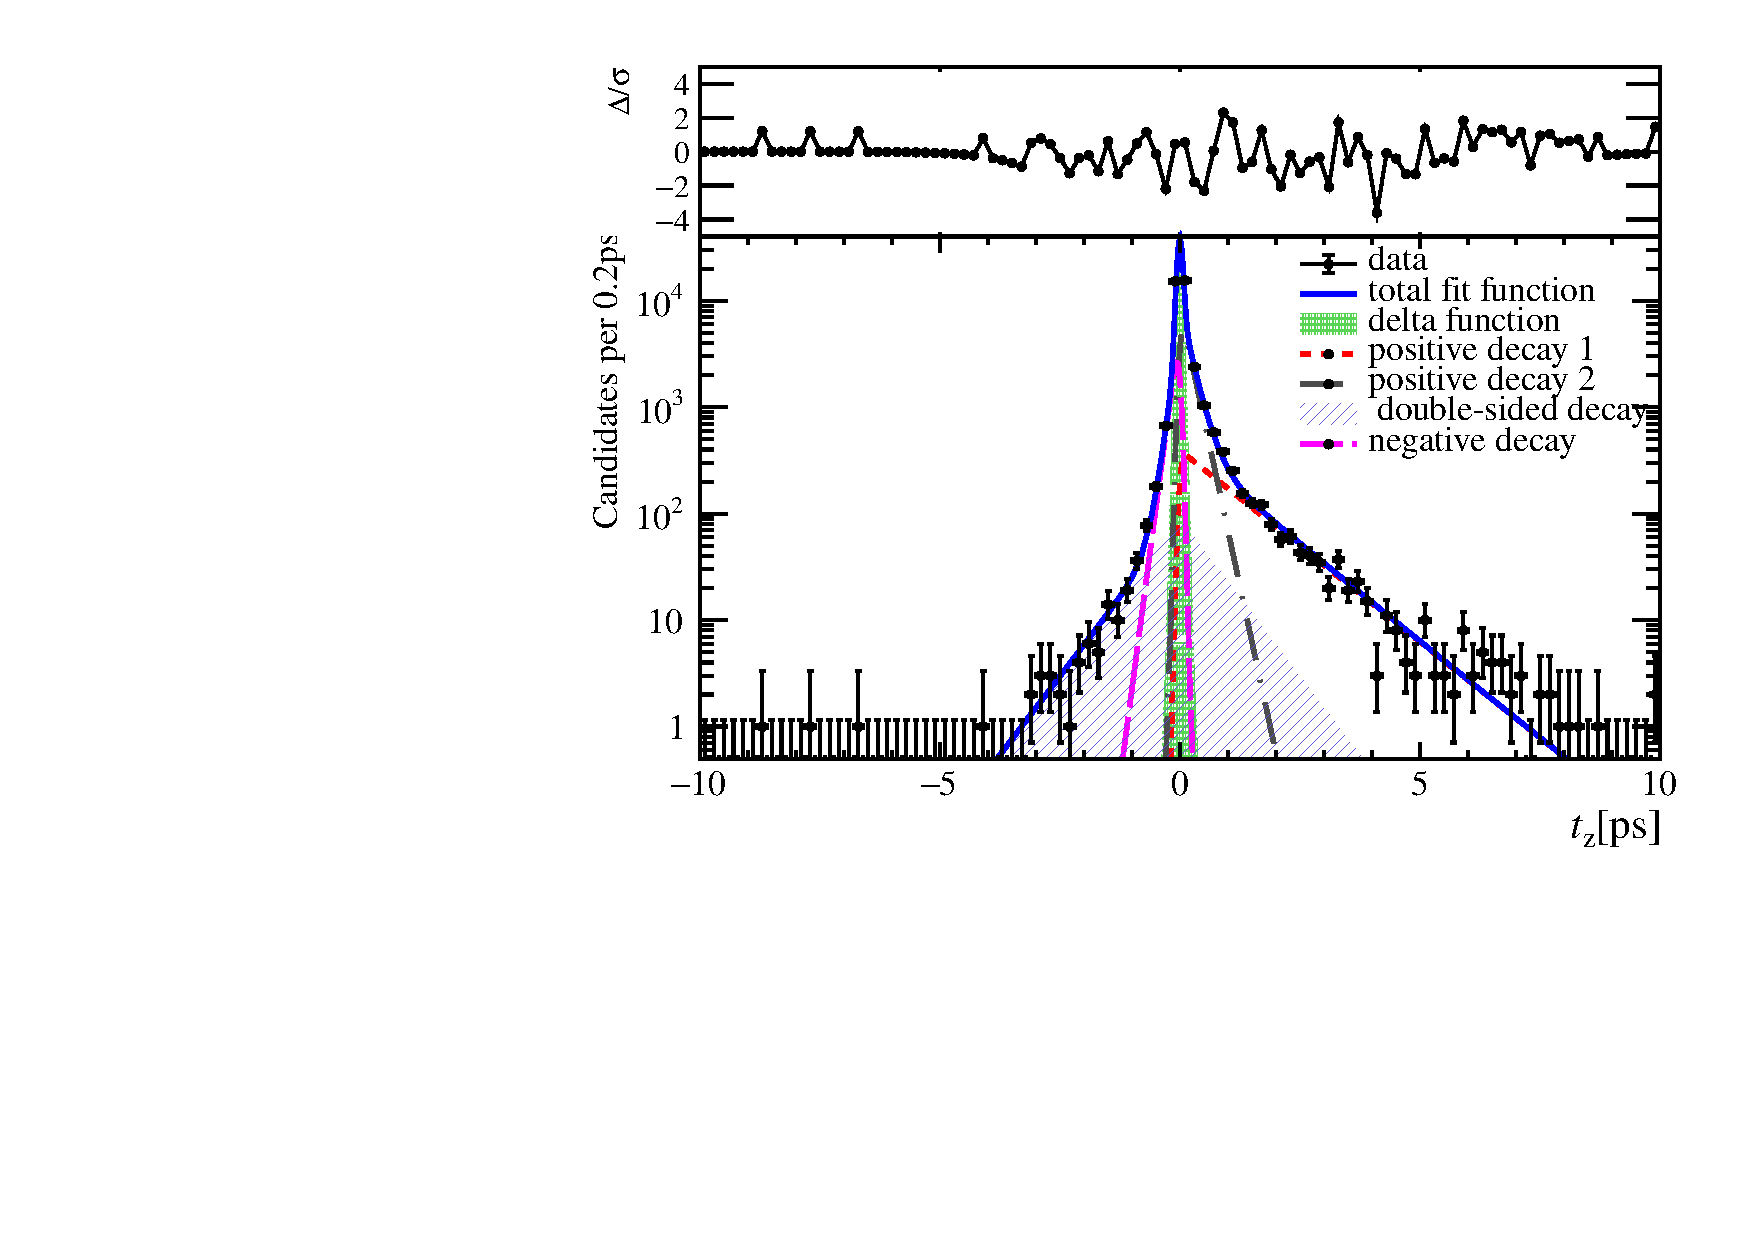
\includegraphics[width=0.49\linewidth]{pdf/Psi2S/Tzbkg/n2y1pt2}
     \vspace*{-0.5cm}
   \end{center}
   \caption{
     $t_z$ background fit for PVNTRACKS from 20 to 40, y from 2 to 2.8, and pt from 2$\gevc$ to 4 $\gevc$. The left is that of $\jpsi$ and the right is of $\psitwos$.
     }
   \label{fig:TzBKG}
 \end{figure}
%%%%%%%%%%%%%%%%%%%%%%%%%%%%%%%%%%%%%%%%%%%%%%%%%%%%%%%%%%
In total, the eventual function for the $t_z$ fit is:
\begin{align}
F_{t_z}(t_z;n_{\mathrm{prompt}},n_{tail},n_{\mathrm{bdecay}},n_\mathrm{bkg},\mu,S_1,S_2,\beta,\tau_b)&   \nonumber \\
      =\left(n_{\mathrm{prompt}}\delta(t_z)+\frac{n_{\mathrm{bdecay}}}{\tau_b}e^{-t_z/\tau_b}\right)\ast f_\mathrm{resolution}(t_z;\mu,S_1,S_2,\beta)
      &+n_{\mathrm{tail}} f_\mathrm{tail}(t_z)+n_\mathrm{bkg}f_\mathrm{background}(t_z), \label{eq:FinalTz}
\end{align}
where $n_\mathrm{bkg}$, $n_{\mathrm{prompt}}$, $n_{\mathrm{bdecay}}$ and $n_{\mathrm{tail}}$ are the number of background, prompt components, components from $\bquark$ and wrong PV events, respectively. 

Because the requirement of the PV reconstruction is loose, and the PV is not refitted by removing the VELO segments of the muon tracks, it is reasonable to assume that prompt components and components from $\bquark$ have equal probability to be assigned with a wrong PV.
Therefore, the fractions of the prompt and from $\bquark$ components in $n_{\mathrm{tail}}$ is equal to the fraction $\frac{n_{\mathrm{prompt}}}{n_{\mathrm{bdecay}}+n_{\mathrm{prompt}}}$ and $\frac{n_{\mathrm{bdecay}}}{n_{\mathrm{bdecay}}+n_{\mathrm{prompt}}}$. 
Even if the shape is extracted from data including the background candidate, the fit result $n_{\mathrm{tail}}$ should only contain prompt and non-prompt signals. First, the shape of the PDF due to the wrong-PV effect should be the same no matter from which sample we extract it. Then, 
the wrong-PV effect for background candidates should be merged in the background PDF, which means the $n_{\mathrm{tail}}$ part in the total PDF should be specifically for signal candidates.
And in this analysis, we only care about the ratio of prompt and from $\bquark$, where $n_{tail}$ in each kinetic bin and multiplicity bin accounts for about $0.1\%$ of $n_{\mathrm{bdecay}}+n_{\mathrm{prompt}}$, which results in an even more negligible influence on the ratio in Sec~\ref{Ratio of Cross-Section Determination}. 
In this case, we can ignore the subtle contribution to $n_{\mathrm{bdecay}}$ and $n_{\mathrm{prompt}}$ from $n_{tail}$. 

The two-dimensional fit to the invariant mass and the lifetime in the kinematic range $4\gevc<\pt<6\gevc$, $2.0<y<2.8$ 
and multiplicity bin 20$\leq$PVNTRACKS$<$40 is shown in Fig.~\ref{fig:2Dtz}, with the red shaded area being prompt components, and the cyan shaded area being components from $\bquark$, 
the dots with vertical error bar are data points, the violet dashed lines are the combinatorial background, the green dashed lines are the components by wrong PV (which are invisible in the graph of projection on mass) and 
the blue lines are the total fit functions.
During the $t_z$-mass combined fitting procedure, the parameters of mass signal shape ($\mu_{mass}$, $\sigma_{mass}$, $p_{0}$) are floated within a certain times of their uncertainties from the 1D mass fit for the final fits of \jpsi. While for \psitwos, due to the limitation of number of candidates, the parameters are fixed. According to the comparison of two fitting strategies upon \jpsi, no significant difference between errors of prompt and non-prompt signals are observed (~$0.1\%$).
%The $t_z$-mass combine fitted value $\beta$ (fraction of first Gaussian of signal resolution function),  $1000*\mu_{t_z}$ (bias of $t_z$ distribution), $S(1,2)_{t_z}$ ($\sigma_{1,2}$ of first/second Gaussian resolution function convolved with the $t_z$ function), $\tau_b$(effective $b$-hadron lifetime), $n_\mathrm{bkg}$, $n_{prompt}$ (number of prompt \psitwos), $n_{b-decay}$ (number of \psitwos-from-\bquark) and $n_{tail}$ (number of events in tail) are given in Tables\ref{tab:FitResults0}, \ref{tab:FitResults1}, \ref{tab:FitResults2}, \ref{tab:FitResults3} and \ref{tab:FitResults4}. 

 %%%%%%%%%%%%%%%%%%%%%%%%%%%%%%%%%%%%%%%%%%%%%%%%%%%%%%%%%%%
 \begin{figure}[!tbp]
   \begin{center}
     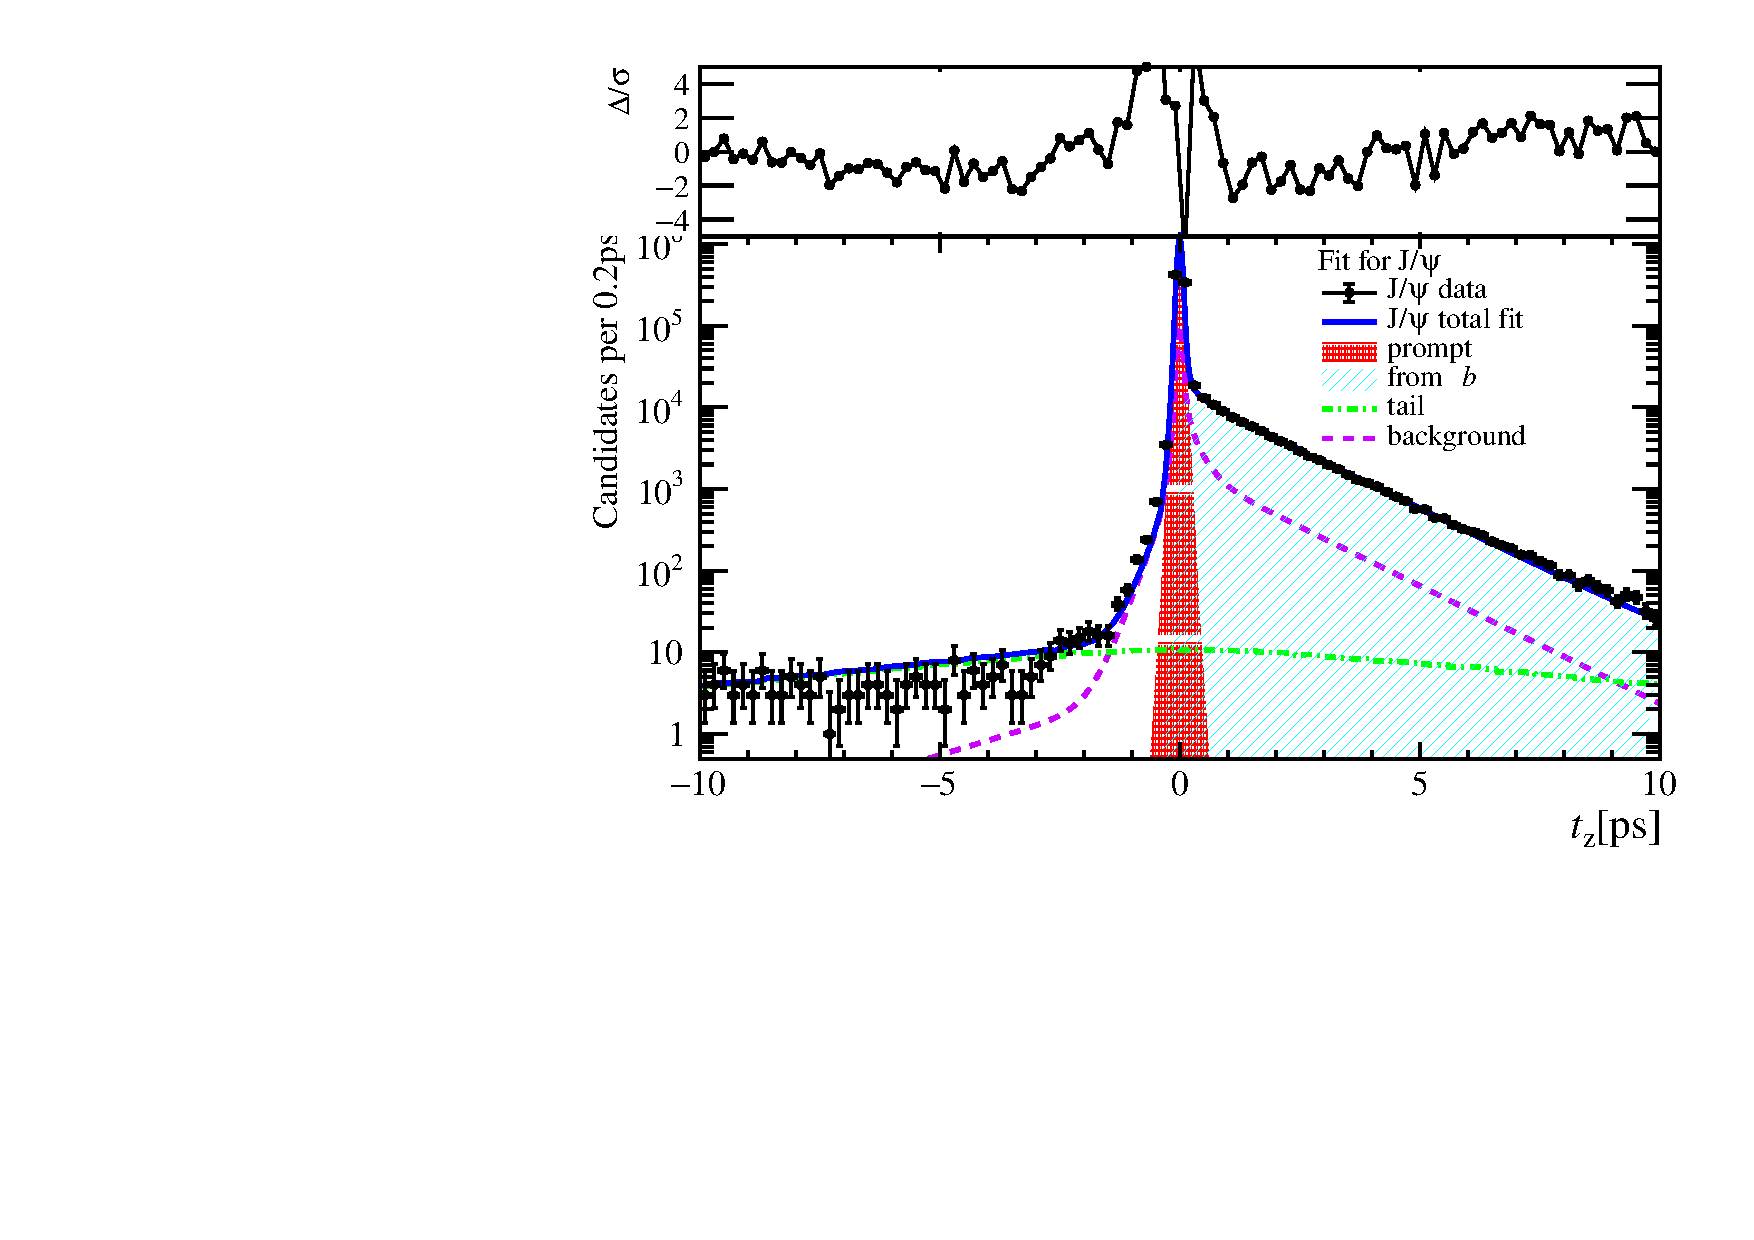
\includegraphics[width=0.49\linewidth]{pdf/Jpsi/2DFit/n2y1pt2.pdf}
     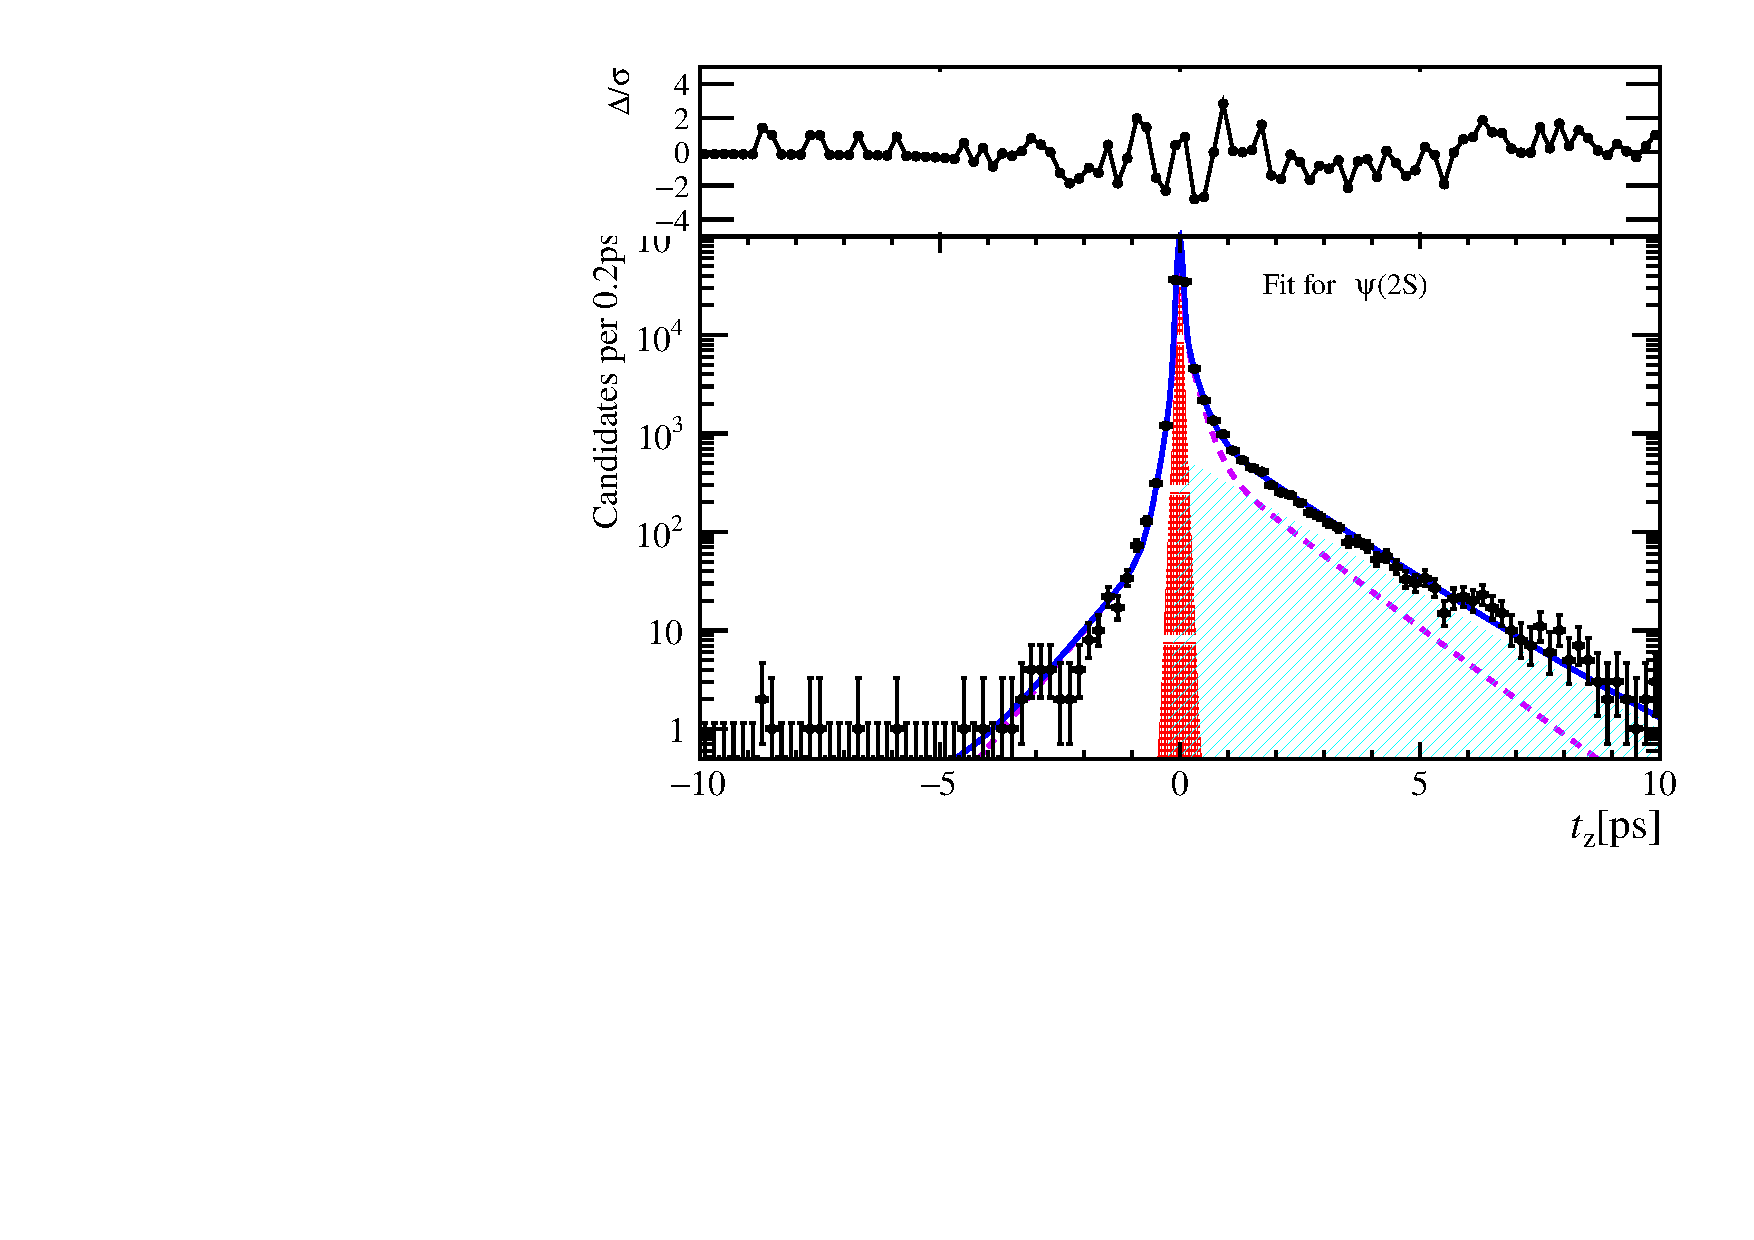
\includegraphics[width=0.49\linewidth]{pdf/Psi2S/2DFit/n2y1pt2.pdf}
     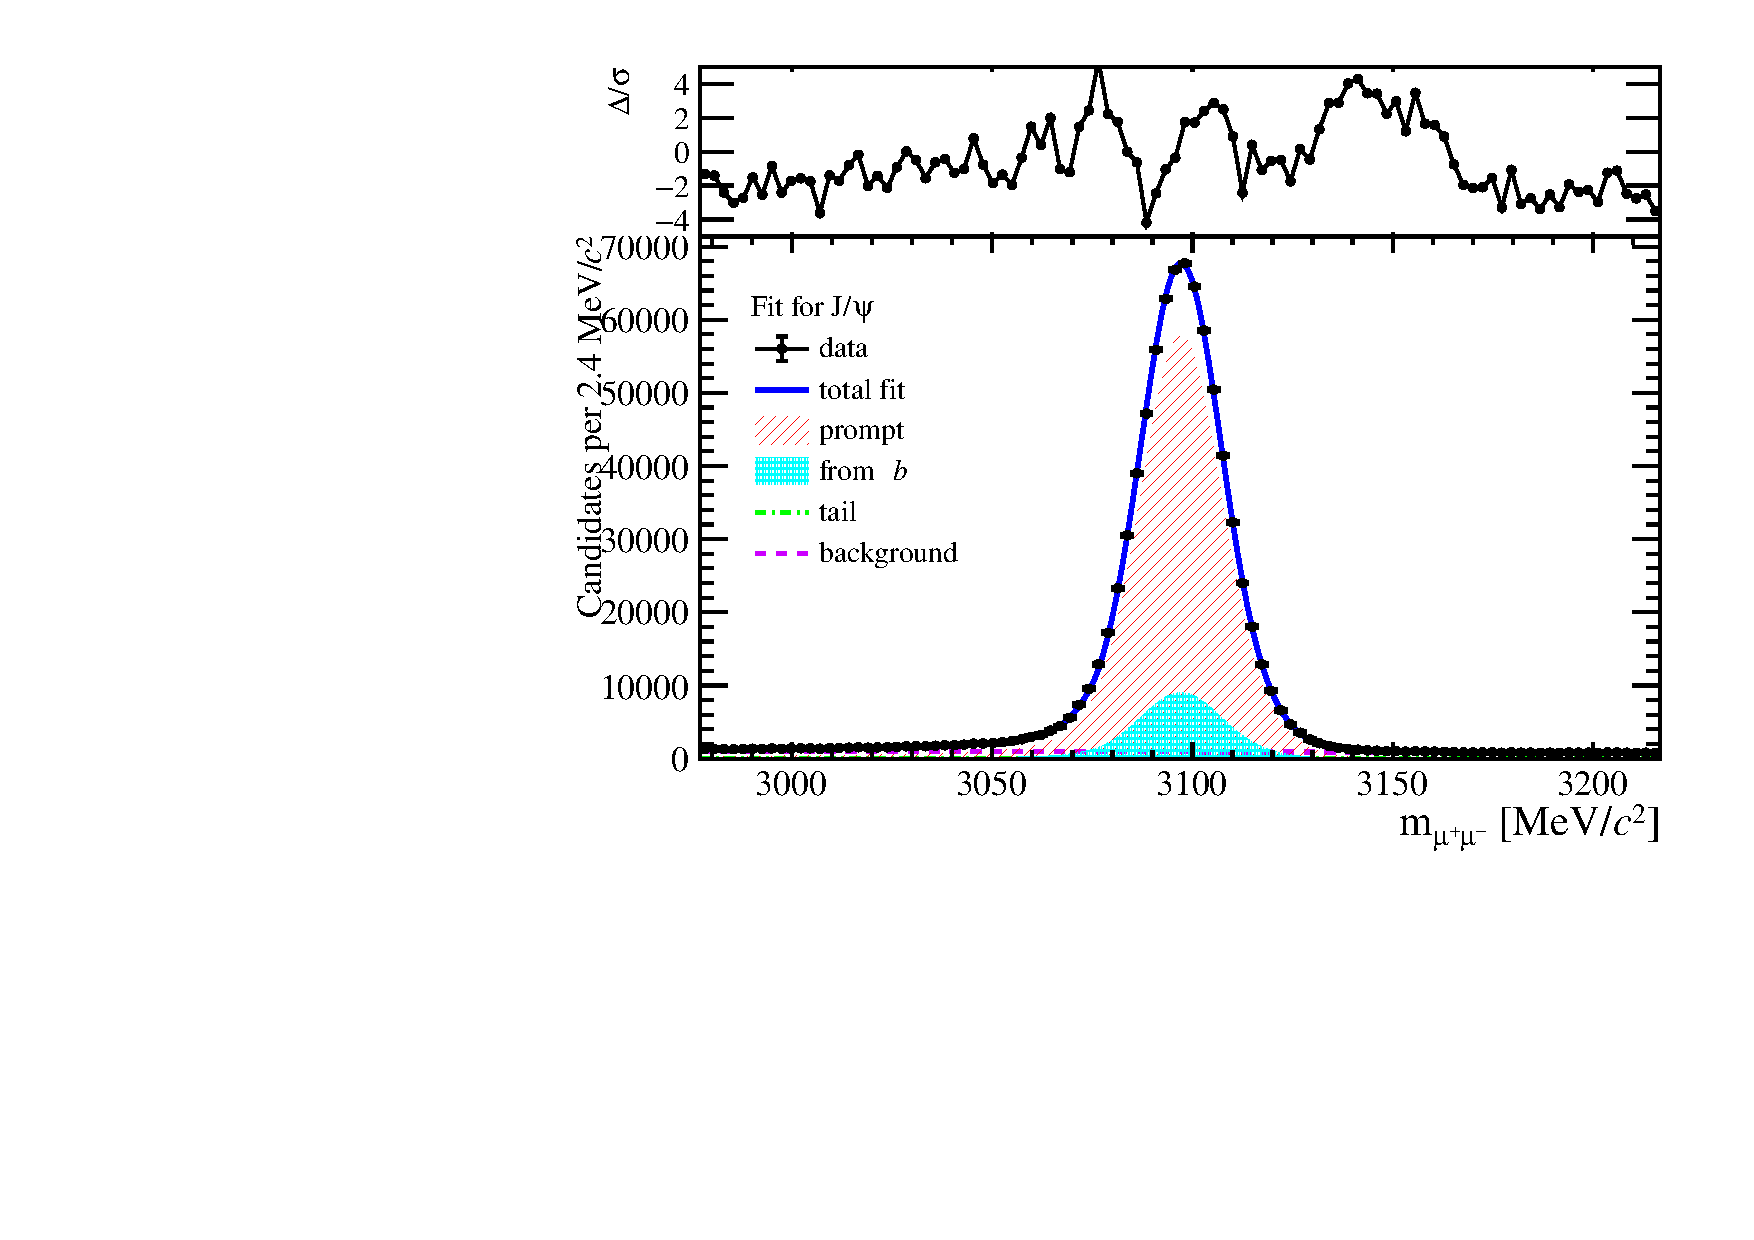
\includegraphics[width=0.49\linewidth]{pdf/Jpsi/drawmass/n2y1pt2.pdf}
     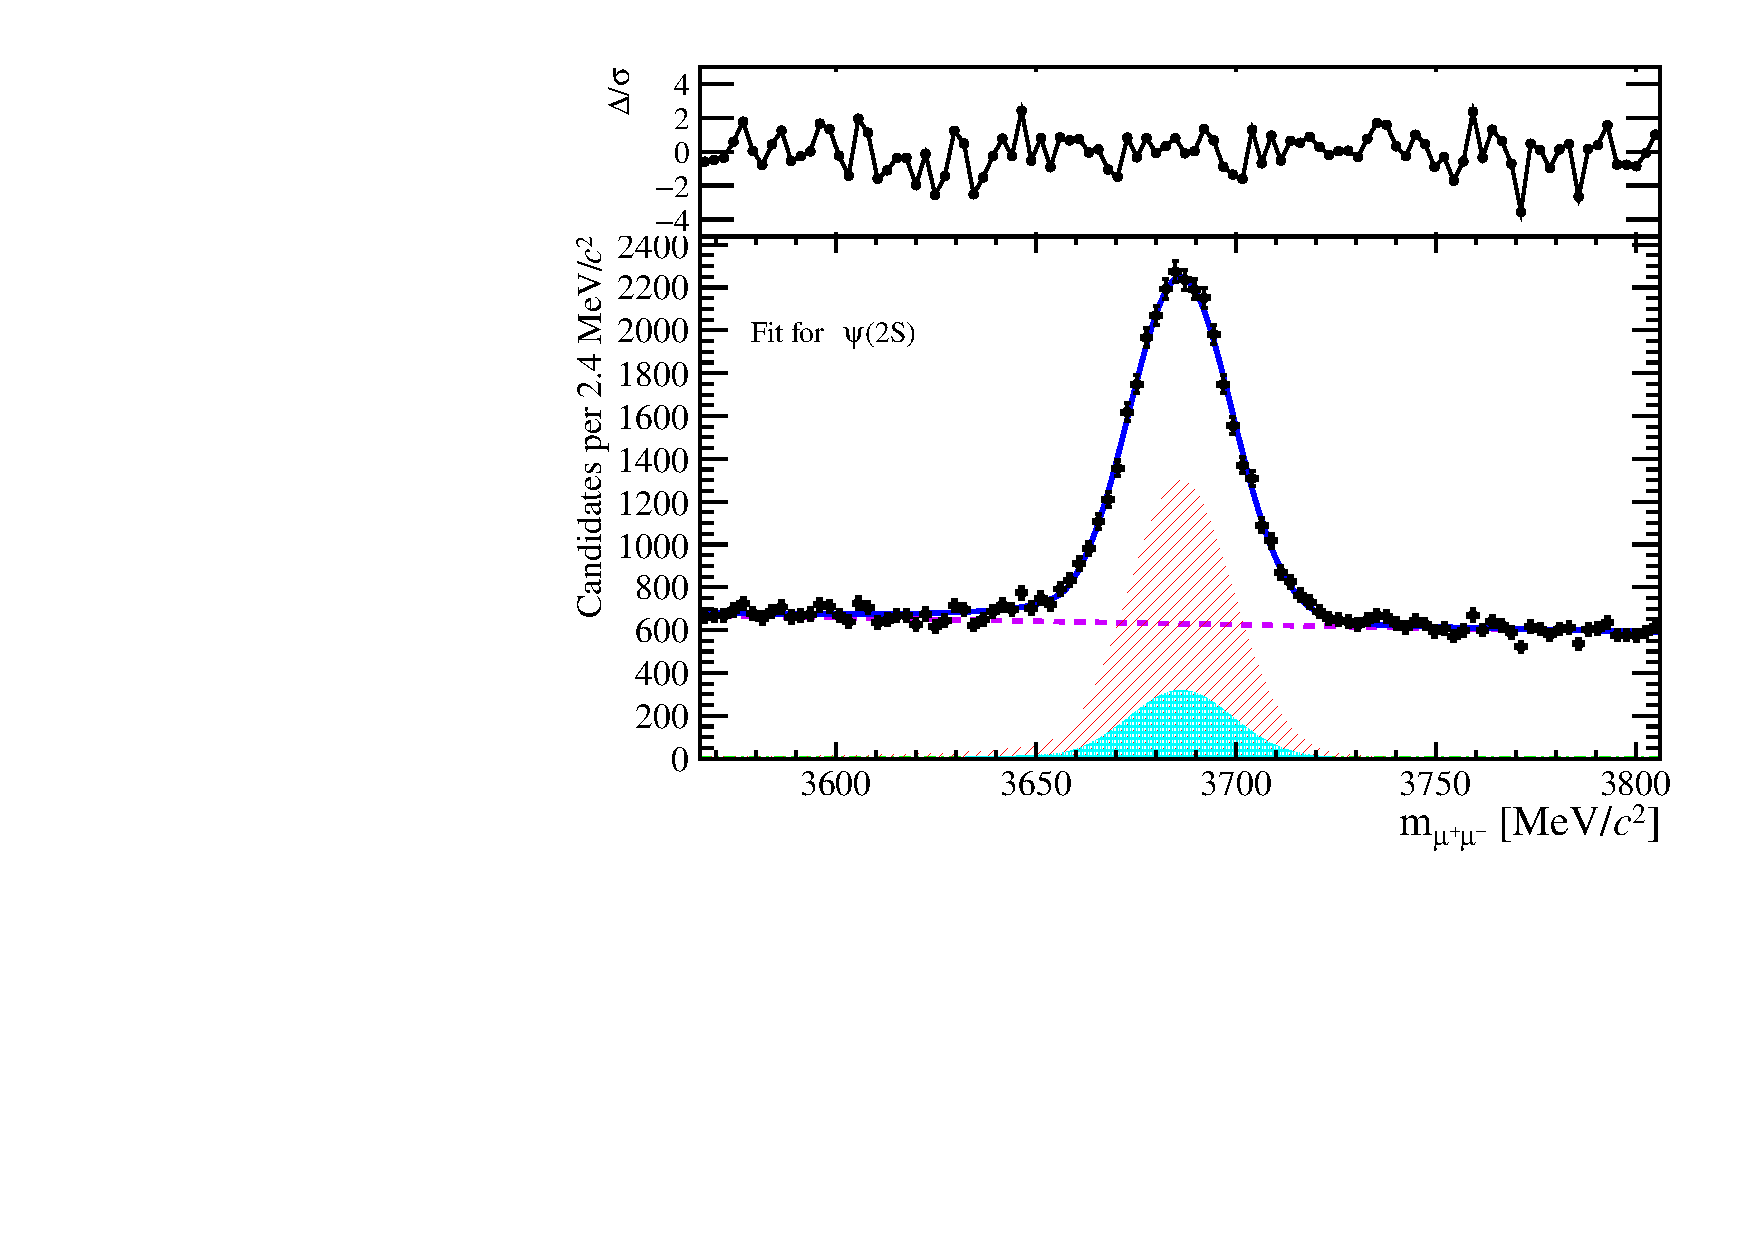
\includegraphics[width=0.49\linewidth]{pdf/Psi2S/drawmass/n2y1pt2.pdf}
   \end{center}
   \caption{
     Projection in $t_z$ and mass spectrum of $t_z$-mass fit for PVNTRACKS from 20 to 40, y from 2 to 2.8, and pt from 2$\gevc$ to 4 $\gevc$. The left is that of $\jpsi$ and the right is of $\psitwos$.
     }
   \label{fig:2Dtz}
 \end{figure}
%%%%%%%%%%%%%%%%%%%%%%%%%%%%%%%%%%%%%%%%%%%%%%%%%%%%%%%%%%%

